\documentclass{beamer}
\usepackage[utf8]{inputenc}
\usepackage[english]{babel}
\setbeamersize{text margin left=10pt, text margin right=10pt} %new code
\usepackage{graphicx}
\usepackage{float}
\usepackage{animate}
\usepackage{movie15}
\usepackage{breqn}
\usepackage{tcolorbox, amsmath}
\usepackage{subcaption}
\newcommand{\mysetminus}{\mathbin{\fgebackslash}}

\setbeamerfont{headline}{size=\small}


%----------------------------------------------------------------------------------------
%	 Package
%----------------------------------------------------------------------------------------
\usepackage{color}
\usepackage{url}
\usepackage{minted}		% listing code
\beamertemplatenavigationsymbolsempty

\definecolor{cadmiumred}{rgb}{0.8, 0.8, 0.8}

%----------------------------------------------------------------------------------------
%	 Presentation settings
%----------------------------------------------------------------------------------------

\usetheme{CambridgeUS}
\usecolortheme{beaver}


\setbeamertemplate{itemize items}[triangle] 
\setbeamertemplate{enumerate items}[default]
 
\title[Deeep Structured Models]{Scientific Seminar "Bayesian Methods of ML"\\
	\vspace{1cm}
	\textbf{\textcolor{black}{Deep Structured Models}}}

\author{Ashuha Arseniy}
\institute[MIPT]{
	Moscow Institute of Physics and Technology
	
	\medskip
	
	\href{mailto:ars.ashuha@gmail.com}{\nolinkurl{ars.ashuha@gmail.com}}}

\date{\today}

\newcommand{\Expect}{\mathsf{E}}
\newcommand{\MExpect}{\mathsf{M}}
\newcommand{\cov}{\mathsf{cov}}


\begin{document}
%----------------------------------------------------------------------------------------
%	 Title
%----------------------------------------------------------------------------------------
\begin{frame}
	\titlepage 
	\footnotesize{Based on article:  \emph{Chen, Schwing, et al. "Learning deep structured models." ICML 2015}}
\end{frame}

\section{Neural Nets and Graphical Models}
\frame{\tableofcontents[currentsection]}

\subsection*{Deep Neural Nets}
\begin{frame}
	\centering 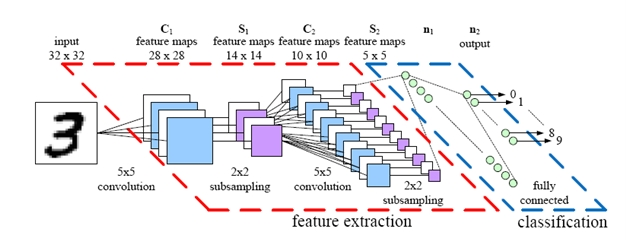
\includegraphics[scale=0.5]{img/dnn} 
	
	\begin{itemize}
		\item \textbf{NNs} is a framework for constructing flexible models
		
		\item Neural net is a \textbf{composition} linear and nonlinear functions 	
			\vspace{0.1cm}
			\begin{center}
				\Large $argmax(\sigma[Linear(\sigma[Linear($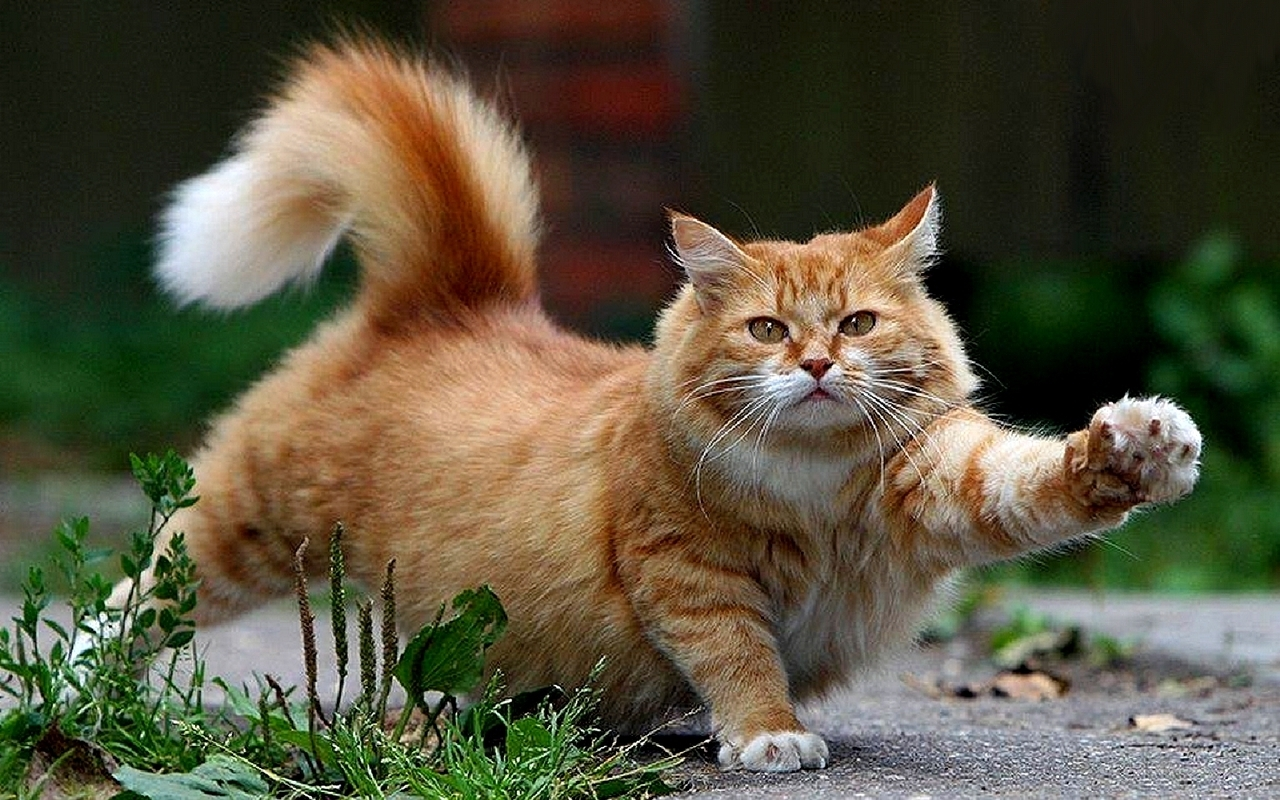
\includegraphics[scale=0.03]{img/cat}$, w)], w)])$ = cat
			\end{center}
			\vspace{0.1cm}
		
		\item \textbf{We can learn it efficiently} by back propagation
		\end{itemize}

	
		\begin{tcolorbox}[colback=gray!2, colframe=red!90, title=Problem]
			\centering Can't take into account dependences between predicted variables. 
		\end{tcolorbox}
\end{frame}

\subsection*{Structured Prediction}
\begin{frame}
	\begin{itemize}
		\item Non structured -- predict simple variable (like a number)
		\item Structured -- predict difficult variable (like a matrix, tree, sequence)
	\end{itemize}
	
	\begin{figure}
		\begin{subfigure}{.49\textwidth}
			\centering 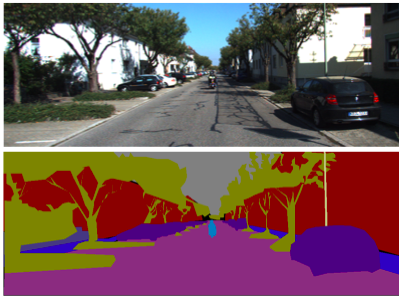
\includegraphics[scale=0.23]{img/seg} 
			\caption{Segmentation, $|Y| = \#pixel^{\#sigment}$}
		\end{subfigure}
		\begin{subfigure}{.49\textwidth}
			\centering 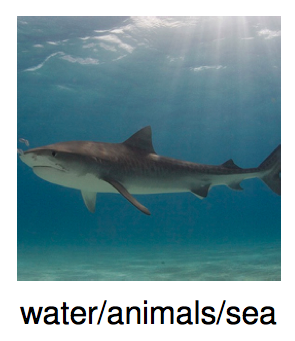
\includegraphics[scale=0.2]{img/taging} 
			\caption{Tagging, $|Y| = 2^{\#tags}$}
		\end{subfigure}
		
		\vspace{0.2cm}
		
		\begin{subfigure}{.49\textwidth}
			\centering  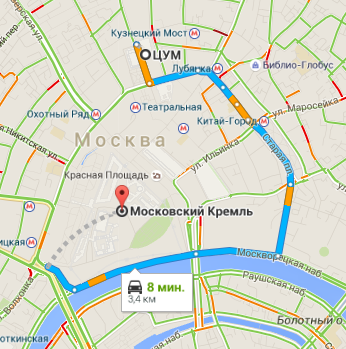
\includegraphics[scale=0.2]{img/trafic} 
			\caption{Traffic prediction, $|Y| = ?$}
		\end{subfigure}
		\begin{subfigure}{.49\textwidth}
			\centering 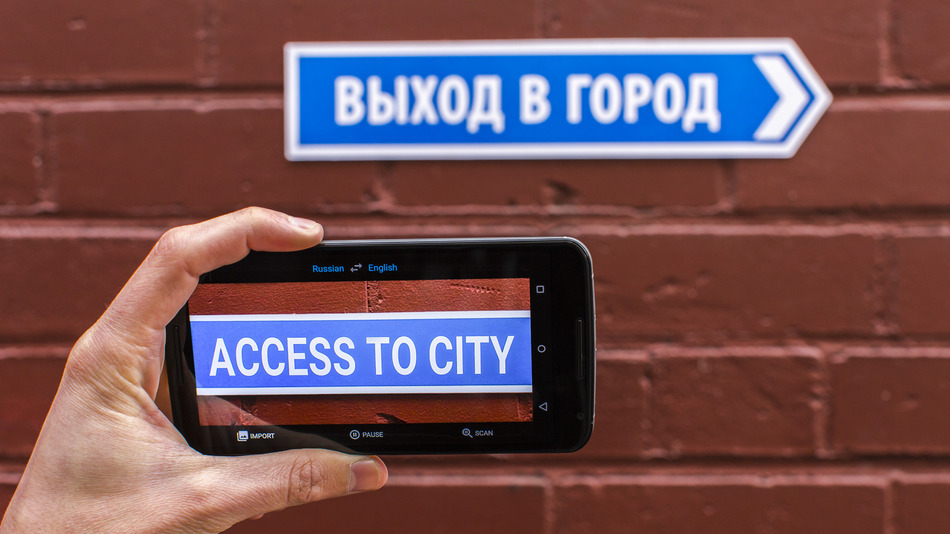
\includegraphics[scale=0.18]{img/transl} 
			\caption{Translation, $|Y| = ?$}
		\end{subfigure}
	\end{figure}
\end{frame}

\subsection*{Graphical Models}
\begin{frame}
	\begin{itemize}
		\item \textbf{GMs} is a framework for taking into account dependencies between predicted variables.
		\item What can we do with exp-large output space? Use local dependences.
		\item Introduce prior knowledge as a score functions $\phi_r(y_r)$, $|y_r|$ is small
			\begin{columns}[onlytextwidth]
				\begin{column}{0.5\textwidth}
					\begin{center}
						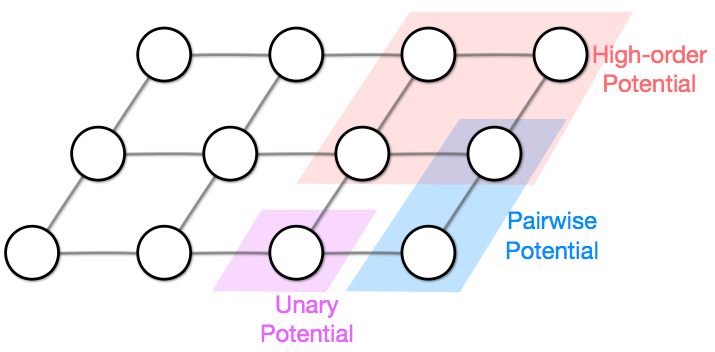
\includegraphics[scale=0.18]{img/gm}
					\end{center}
				\end{column}
				\begin{column}{0.50\textwidth}
					$\phi_{y1, y2}(people, male) = 10$ is high 
					
					$\phi_{y1, y2}(wather, girl) = 0.2$ is low			
					
					....
				\end{column}
			\end{columns}
			
		\item We can introduce non-normalized probability distribution over outputs
			$$p(y|x, w) = \frac{1}{Z} \prod_r \phi_r(x, y_r; w)~~~~~~Energy = - \sum_r \phi_r(x, y_r; w)$$
		
		\item \textbf{Inference Task}: 
			$$y^\star = \arg\max_y p(y|x, w)$$
	\end{itemize}
\end{frame}

\subsection*{Log-linear restrictions [Raquel slides !!!]}
	\begin{frame}
		\begin{enumerate}
			\item We want to \textbf{train parameters} $w$ of parametric potential 
			\item Given training data $(x, y) \in D$; estimate the functions $f_r(y,x,w)$
			\item Minimize a typically convex loss and a regularize on training set
				$$Loss_{log}(x, y, w) = - \ln~p_{x, y}(y; w)$$
				$$Loss_{hinge}(x, y, w) = \max_{\hat{y}} (\Delta(y, \hat{y}) - w^T\Phi(x, \hat{y}) + w^T\Phi(x, y))$$
			\item The assumption is that the model is \textcolor{red}{log-linear}
				$$E(x,y,w) = - w^T \phi(x,y)$$
			and the features decompose in a graph
				$$w^T\phi (x, y) = \sum_{r \in R} w_r^t\phi( x , y )$$
		\end{enumerate}
			\begin{tcolorbox}[colback=gray!2, colframe=red!90, title=Problem]
				\centering How can we remove the log-linear restriction, 
				
				to use potentials such as Neural Nets? 
			\end{tcolorbox}
	\end{frame}

\section{Deep Structured Models}
\frame{\tableofcontents[currentsection]}

\subsection*{Intuition}
\begin{frame}
	How can we combine Graphical Models and Deep Neural Nets? 
	\begin{enumerate}
		\item Peace-wise learning:
			\begin{itemize}
				\item train deep features $\rightarrow$ train linear potential $\rightarrow$ inference in GM
			\end{itemize}
		\item Jointly learning:
			\begin{itemize}
				\item train deep features as non linear potential $\rightarrow$ inference in GM
			\end{itemize}
	\end{enumerate}
	
	\onslide<1>{\centering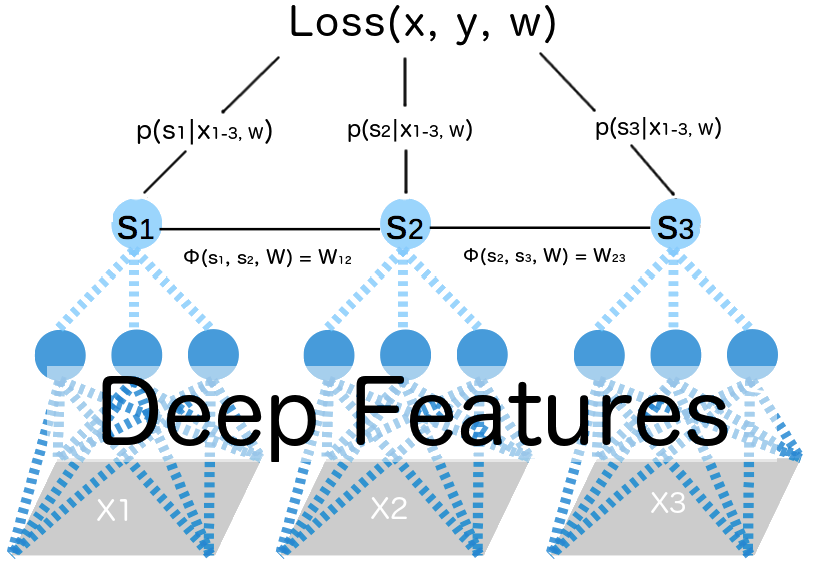
\includegraphics[scale=0.25]{img/dsm1}}
	\onslide<2>{\vspace{-5.1cm}
		
		\centering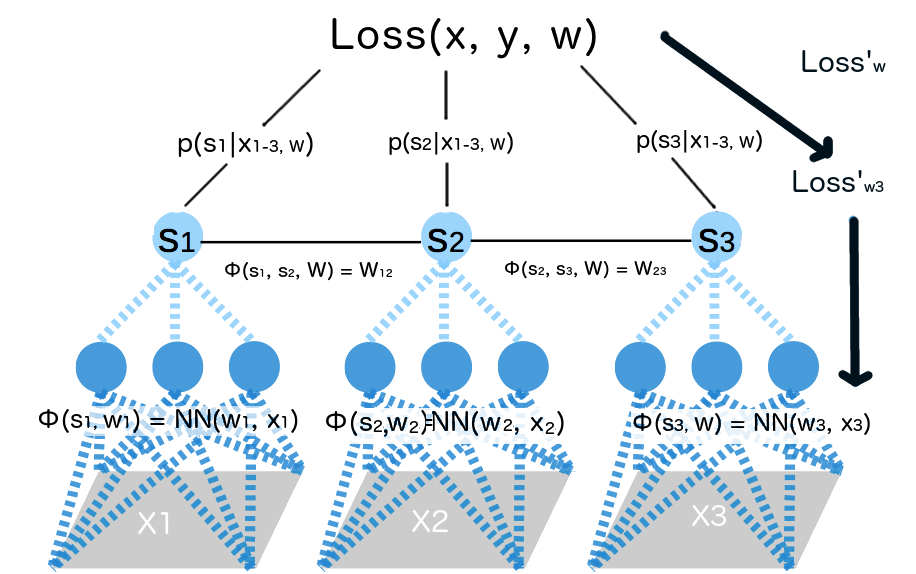
\includegraphics[scale=0.25]{img/dsm2}}
\end{frame}

\subsection*{Definitions [Chen slides]}
\begin{frame}
	\begin{itemize}
		\item We have: scoring function $F(x, y; w)$, training data $(x, y) \in D$
	
		\item \textcolor{red}{Prediction proses} is equal finding maximum scoring configuration $y^\star$:
		
		$$y^\star = arg\max_{y} F(x, y; w)$$
		\item Introduce probability distribution over configurations as
		
		$$p_{(x, y)}(\hat{y}|w) = \frac{exp~F(x, \hat{y}, w)}{\sum_{y'} exp~F(x, y', w)} = \frac{exp~F(x, \hat{y}, w)}{Z(x, w)}$$
		rephrase previous task as finding high probably configuration
		\item \textcolor{red}{Training proses} is finding parameters $w$ by MLE
		
		
		\begin{center}
			$w = \arg\max_{w}log\prod_{(x, y) \in D} p_{(x, y)}(y|w) = $
			
			\vspace{0.2cm}
			
			$= \arg\max_{w}\sum_{(x, y) \in D} F(x, y, w) - ln~Z(x, w) $
		\end{center}	
	\end{itemize}
\end{frame}

\subsection*{Simple solution [Chen slides]}
\begin{frame}
	
	We have optimization problem:
		$$\sum_{(x, y) \in D} \left(F(x, y, w) - log~\sum_{y' \in Y} exp~F(x, y', w)\right) \rightarrow \max_{w}$$
	Let's solve it by gradient assent \small{\textcolor{gray}{(will be proof on the board if it's necessary)}}:
	$$\frac{\partial}{\partial w} \sum_{(x, y) \in D} \left( F(x, y, w) - logZ(x, w) \right) =$$
	
	$$= \sum_{(x, y) \in D} \sum_{y' \in Y} (\textcolor{black}{p(y'|w, x)} - \delta(y'=y)) \frac{\partial}{\partial w} F(x, y', w)$$ 
	
	\begin{center}
		\textbf{Very easy! Where is a challenge?}		
		
		\begin{tcolorbox}[colback=gray!2, colframe=red!90, title=Problem: What If Y is exponentially large!]
			1) \textcolor{black}{How can we represent F?}~~~2) What we can do with sum over Y?
		\end{tcolorbox}
	\end{center}
\end{frame}

\subsection*{Approximate Learning [Chen slides]}

\begin{frame}
	$$\sum_{(x, y) \in D} \left(F(x, y, w) - log~\sum_{y' \in Y} exp~F(x, y', w)\right) \rightarrow \max_{w}$$
	\begin{enumerate}
		\item Use the graphical model $F(x, y; w) = \sum_{r} f_r(x, y; w)$
			$$\frac{\partial}{\partial w} \sum_{(x, y) \in D} \left( F(x, y, w) - logZ(x, w) \right) =$$
			$$= \sum_{(x, y) \in D} \sum_{y' \in Y} (\textcolor{black}{p(y'|w, x)} - \delta(y'=y)) \frac{\partial}{\partial w} F(x, y', w)$$ 
			\small{\textcolor{gray}{(will be proof on the board if it's necessary)}}:
			$$= \sum_{(x, y) \in D} \sum_{y'_{\textcolor{red}{r}}, {\textcolor{red}{r}}} (\textcolor{black}{p_{ {\textcolor{red}{r}}}(y'_{\textcolor{red}{r}}|w, x)} - \delta(y'_{\textcolor{red}{r}}=y_{\textcolor{red}{r}})) \frac{\partial}{\partial w} f_{\textcolor{red}{r}}(x, y'_{\textcolor{red}{r}}, w)$$ 
			
		\item How to obtain marginals $p_r(y_r|w, x)$?
		\item Use beliefs  $p_{r}(y_r|w, x) \approx b_{r}(y_r|w, x)$
	\end{enumerate}
	

\end{frame}


\subsection*{Learning DSM (algo 1) [Raquel slides]}
\begin{frame}
	\begin{tcolorbox}[colback=white!2, colframe=gray!90, title=Deep Structured Learning (algo 1)]
		Repeat until stopping criteria:
		\begin{enumerate}
			\item Forward pass to compute the $f_r(y_r , x; w)~~~~~~~\forall r, y_r, (x, y) \in D$
			\item Compute the $b_r(y_r | x, w)$ by approx inference $~\forall r, y_r, (x, y) \in D$
			\item Backward pass via chain rule to obtain gradient
			$$\frac{\partial}{\partial w}= \sum_{(x, y) \in D, y'_{\textcolor{black}{r}}, {\textcolor{black}{r}}} (\textcolor{black}{b_{{\textcolor{black}{r}}}(y'_{\textcolor{black}{r}}|w, x)} - \delta(y'_{\textcolor{black}{r}}=y_{\textcolor{black}{r}})) \frac{\partial}{\partial w} f_{\textcolor{black}{r}}(x, y'_{\textcolor{black}{r}}; w)$$ 
			\item Update parameters w 
				$$w = w  - \alpha \cdot \partial/\partial w$$
		\end{enumerate}
	\end{tcolorbox}
	
	\begin{tcolorbox}[colback=gray!2, colframe=red!90, title=Problem]
		\centering We run inference  for each object to make one parameters update
	\end{tcolorbox}
\end{frame}

\section{Efficient Approximate Learning of DSM}
	\frame{\tableofcontents[currentsection]}
	
\subsection*{LP-relaxation}

\begin{frame}
	\begin{tcolorbox}[colback=white!2, colframe=red!90]
		$$\sum_{(x, y) \in D} \left( F(x, y, w) - log~\sum_{y' \in Y} exp~F(x, y', w) \right) \rightarrow \max_{w}$$
	\end{tcolorbox}
	
	\begin{enumerate}
		\item We can represent Z as \small \textcolor{gray}{(will be proof on the board if it's necessary)}:
			$$ln~Z = \sum_{\hat{y}} exp~F(x, \hat{y}, w) = \max_{p_{(x, y)}} \mathbb{E}_{p_{(x, y)}(\hat{y})} F(x, \hat{y}; w) + H(p_{(x, y)})$$
		
		\item Assumption, F and H is decomposed into a sum of "local" functions \small
		$$F = F(x, y; w) = \sum_{r} f_r(x, y_r; w)~~~~H = H(p_{(x, y)}) = \sum_{r} H(p_{(x, y), r})$$
		
		\item Rephrase our task as
		$$\min_w \sum_{(x, y) \in D} \left(\max_{p_{(x, y)}} \left\{ \sum_r p_{(x, y), r} (\hat{y}_r) f_r(x, \hat{y_r}; w) + H(p_{(x, y)})\right\}- F \right) $$
		
	\end{enumerate}
\end{frame}

\subsection*{Approximate marginal distributions}
 \begin{frame}
	\begin{tcolorbox}[colback=white!2, colframe=red!90]
		\vspace{-0.5cm}
		$$\sum_{(x, y) \in D} \left(\max_{p_{(x, y)}} \left\{ \sum_r p_{(x, y), r} (\hat{y}_r) f_r(x, \hat{y}_r; w) + H(p_{(x, y)})\right\}- F \right) \rightarrow \min_w$$
	\end{tcolorbox}
 		
 	\begin{enumerate}
 		\item We can't compute true marginals, let's use  beliefs $b_{(x, y)} \approx p_{(x, y)}$
	 		{\small
	 		$$b_{(x, y)} \in C_{(x, y)} = 
		 		\begin{cases} 
			 		b_{(x, y), r}(\cdot) \geq 0~~\sum_{y_r} b_{(x, y), r}(y_r) = 1 ~~~~~ \forall r\\  
				 	b_{(x, y), r}  = \sum_{\hat{y}_p \setminus \hat{y}_r} p_{(x, y), p} (\hat{y}_p) ~~~~~~~~~~~~~~ \forall r, \hat{y}_r, p \in P(r)\\  
				 \end{cases}$$} 		
		\item $P(r) = \{p \in Y: r \subset p\}$ and $C(r) = \{c \in Y: r \in P(c)\}$  
 		\item Rephrase our task as
	 		{\small
		 		$$\min_w \sum_{(x, y) \in D} \left( \max_{b_{(x, y)} \in C_{(x, y)}} \left\{ \sum_r b_{(x, y), r} (\hat{y}_r) f_r(x, \hat{y}_r; w) + H(b_{(x, y)})\right\}- F \right) $$}
 	\end{enumerate}
 	
	\begin{tcolorbox}[colback=gray!2, colframe=red!90, title=Problem]
		\centering We need to solve inner problem to compute subgradient!
	\end{tcolorbox}
 \end{frame}
 
 
\subsection*{Move to Dual task}
\begin{frame}
		\begin{tcolorbox}[colback=white!2, colframe=red!90]
			\vspace{-0.5cm}
			$$\min_w \sum_{(x, y) \in D} \left(\max_{b_{(x, y)} \in C_{(x, y)}} \left\{ \sum_r b_{(x, y), r} (y_r) f_r(x, y_r; w) + H(b_{(x, y)})\right\}- F \right) $$
			
			s.t. {\small $b_{(x, y)} \in C_{(x, y)}$} marginalization and discrete distribution conditions 
			{\scriptsize H is redefined as barrier function when argument is not a distribution:}
		\end{tcolorbox}
	
	\begin{enumerate}
	\item The Lagrangian of inner problem is:
	
	$$L_{(x, y)} = \sum_{r, \hat{y}_r} b_{(x, y), r} (\hat{y}_r) \cdot \hat{f}_r(x, \hat{y}_r; w, \lambda)  + H_{barier}$$
	$$\hat{f}_r(x, \hat{y}_r; w, \lambda)  = f_r(x, \hat{y}_r; w)  + \sum_{p \in P(r)} \lambda_{(x, y), p \rightarrow r} (\hat{y_r})- \sum_{c \in C(r)} \lambda_{(x, y), c \rightarrow r} (\hat{y_c})$$
	
	\item Move to dual task by $\lambda$ \small{\textcolor{gray}{($ln~Z = \max_{p_{(x, y)}} \mathbb{E}_{p_{(x, y)}(\hat{y})} F(x, \hat{y}; w) + H(p_{(x, y)})$)}}:
	
	$$\min_{w, \lambda} \sum_{(x, y), r} \ln{\sum_{\hat{y}_r}} exp~\hat{f}_r(x, \hat{y}_r; w, \lambda) - \sum_{(x, y) \in D} F(x, y; w)$$
	\end{enumerate}
	
	
\end{frame}

\section{Blending Learning}
\subsection*{Main Idea [Chen slides]}
\begin{frame}
	\begin{columns}[onlytextwidth]
		\begin{column}{0.48\textwidth}
			Standard learning: 
			\begin{tcolorbox}[colback=gray!20]
			repeat
					\begin{tcolorbox}[colback=red!10]
					repeat 
						
					~~~~update marginals $b_r$
						
					until convergence
					\end{tcolorbox}			
							
					\begin{tcolorbox}[colback=gray!30]
						update parameters w
					\end{tcolorbox}			
					until convergence
			\end{tcolorbox}
		\end{column}
		\begin{column}{0.48\textwidth}
			Blended learning:
			\begin{tcolorbox}[colback=gray!20]
				repeat
				\begin{tcolorbox}[colback=red!10]
					~~
					
					update marginals $b_r$
				
					~~
					\vspace{0.2cm}
				\end{tcolorbox}			
				
				\begin{tcolorbox}[colback=gray!30]
					update parameters w
				\end{tcolorbox}			
				until convergence
			\end{tcolorbox}
		\end{column}
	\end{columns}
	\bigskip
	
	\textbf{Advantage}: 
	
	\centering More frequent parameter updates
	
	\bigskip
	\hrule
	\bigskip
	{\scriptsize Hazan, Schwing, McAllester, Urtasun: Blending Learning and Inference in Structured Prediction}
\end{frame}

\subsection*{Update $w, \lambda$ [Hazan at al. 2013]}
\begin{frame}
	\begin{tcolorbox}[colback=white!2, colframe=red!90]
		\begin{equation*}
			\begin{aligned}
				D(\lambda, w) = \sum_{(x, y), r} \ln{\sum_{\hat{y}_r}} exp\bigl(f_r(x, \hat{y}_r; w) + \sum_{c \in C(r)} \lambda_{(x, y), c \rightarrow r} (\hat{y}_c) -\\
				\sum_{p \in P(r)} \lambda_{(x, y), r \rightarrow p} (\hat{y_r})\bigr) - \sum_{(x, y)} F(x, y; w) \rightarrow \min_{w, \lambda}
			\end{aligned}
		\end{equation*}
	\end{tcolorbox}
	
	\setlength{\leftmargini}{0.5em}
	\begin{itemize}
	\item Optimize by $w$ \small{\textcolor{gray}{(will be proof on the board if it's necessary)}}:
	
		\begin{equation*}
			\begin{aligned}
				\frac{\partial D}{\partial w} = \sum _{(x, y), r, \hat{y}_r} b_{(x, y), r, \hat{y}_r} \frac{\partial}{\partial w} f_r(x, \hat{y}_r; w) + \sum_{(x, y)} \frac{\partial}{\partial w} F(x, y; w)
			\end{aligned}
		\end{equation*}
		
	\item Optimize by $\lambda$ \small{\textcolor{gray}{(will be proof on the board if it's necessary)}}:
	{\scriptsize
		\begin{multline*}
		\hspace{-0.3cm} \mu_{(x, y), p \rightarrow r} (\hat{y}_r) = \ln~
		\sum_{
			\hat{y}_p \setminus \hat{y}_r}
		\exp~
		(
		f_p(x, \hat{y}_p; w) - 
		\sum_{p' \in P(p)} \lambda_{(x, y),  p \rightarrow p'}(\hat{y}_p)
		+ \sum_{r' \in C(p) \setminus r} \lambda_{(x, y),  r' \rightarrow p}(\hat{y}_{r'}) 
		)
		\\
		\hspace{0cm}\lambda_{(x, y), r \rightarrow p}(\hat{y}_r) \propto 
		c_r \cdot (
		f_r(x, \hat{y}_r; w) - 
		\sum_{c \in C(r)}{\lambda_{(x, y), c \rightarrow r}(\hat{y}_c)} + 
		\sum_{p \in P(r)}{\mu_{(x, y), p \rightarrow r}(\hat{y}_r)}
		)
		- \mu_{(x, y), p \rightarrow r} (\hat{y}_r)
		\end{multline*}}
	\end{itemize}
\end{frame}

\subsection*{Efficient Learning DSM (algo 2)}
	\begin{frame}
		
		\begin{tcolorbox}[colback=white!2, colframe=gray!90, title=Efficient Deep Structured Learning (algo 2)]
			{\footnotesize
			Repeat until stopping criteria:
			\begin{enumerate}
				\setlength{\itemindent}{-2em}
				\item Forward pass to compute the $f_r(y_r , x; w)~~~~~~~~\forall r, y_r, (x, y) \in D$
				\item Compute the $b_r(y_r | x, w) = \exp(\hat{f}_r(x, y_r; w, \lambda))~\forall r, y_r, (x, y) \in D, p \in P(r)$
				{\tiny
				$$
				\hspace{-1.2cm}
				\mu_{(x, y), p \rightarrow r} (\hat{y}_r) = \ln{
					\sum_{
						\hat{y}_p \setminus \hat{y}_r}
					{\exp{
							(
							f_p(x, \hat{y}_p; w) - 
							\sum_{p' \in P(p)} \lambda_{(x, y),  p \rightarrow p'}(\hat{y}_p) + 
							\sum_{r' \in C(p) \setminus r} \lambda_{(x, y),  r' \rightarrow p}(\hat{y}_{r'}) 
							)
						}}}
				$$
				$$
					\hspace{-0.7cm}
						\lambda_{(x, y), r \rightarrow p}(\hat{y}_r) \propto 
						c_r \cdot
						\left(
						f_r(x, \hat{y}_r; w) - 
						\sum_{c \in C(r)}{\lambda_{(x, y), c \rightarrow r}(\hat{y}_c)} + 
						\sum_{p \in P(r)}{\mu_{(x, y), p \rightarrow r}(\hat{y}_r)}
						\right)
						- \mu_{(x, y), p \rightarrow r} (\hat{y}_r)
				$$}
				
				\item Backward pass via chain rule to obtain gradient
				$$g = \sum_{(x, y), r, \hat{y_r}} b_{(x, y), r}(\hat{y}_r) \nabla_w  f_r(\hat{y}_r , x; w) - \nabla_w \sum_{(x, y), r} f_r(x, y;w)$$ 
				\item Update parameters w 
				$$w = w  - \alpha \cdot \partial/\partial w$$
			\end{enumerate}
			}
		\end{tcolorbox}
		
	\end{frame}


\section*{Summary of Deep Structured Models}
\subsection*{[Raquel slides]}
\begin{frame}
	\begin{center}
		 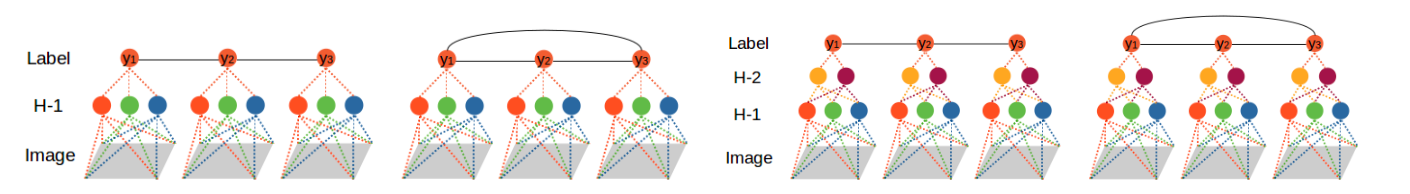
\includegraphics[scale=0.25]{img/dsm_logo}
	\end{center}
	
	\begin{enumerate}
		\item Modeling of correlations between variables
		\item Non-linear dependence on parameters
		\item Joint training of many convolution neural networks
	\end{enumerate}	
\end{frame}

\section{Evaluation}
\frame{\tableofcontents[currentsection]}

\subsection*{Flicker Image Tagging}
\begin{frame}
	\begin{itemize}
		\item \textbf{Task}: Find a combination of tags that describe the image, IYI = $2^{38}$
		\begin{center}
			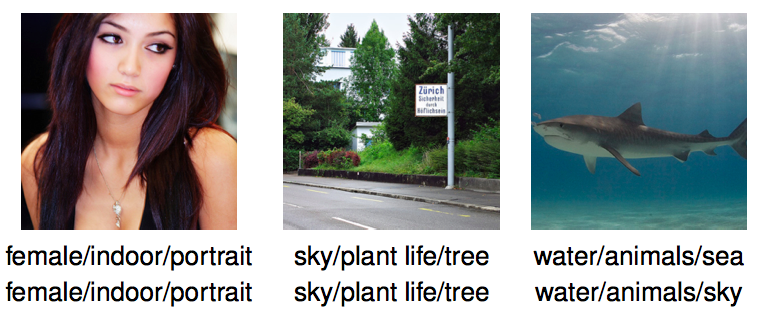
\includegraphics[scale=0.25]{img/flicker1} 
		\end{center}
		
		\item \textbf{Graphical Model}: Fully Connected 38 
		\item \textbf{First order potential}: $f_i(x, y_i; U) = Alexnet(x, U)$
		\item \textbf{Second order potential}: $f_{i, j}(x, y_i, y_j; W) = W_{y_iy_j}$
	\end{itemize}
	
	\begin{center}
		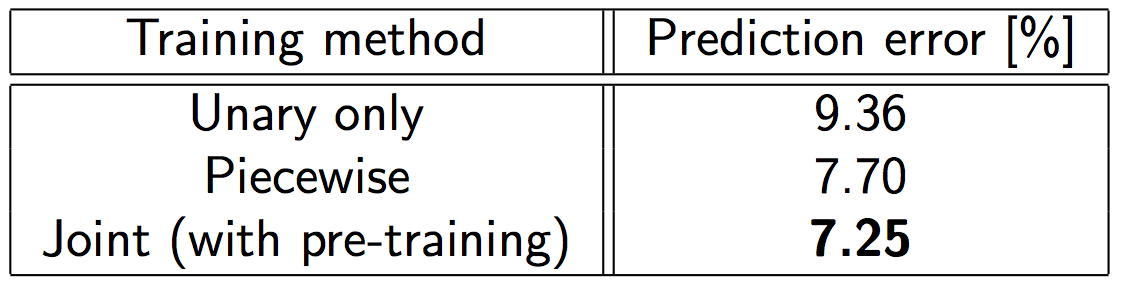
\includegraphics[scale=0.2]{img/flicker2}
	\end{center}
\end{frame}

\begin{frame}
	Learned class "correlations":
	\begin{center}
		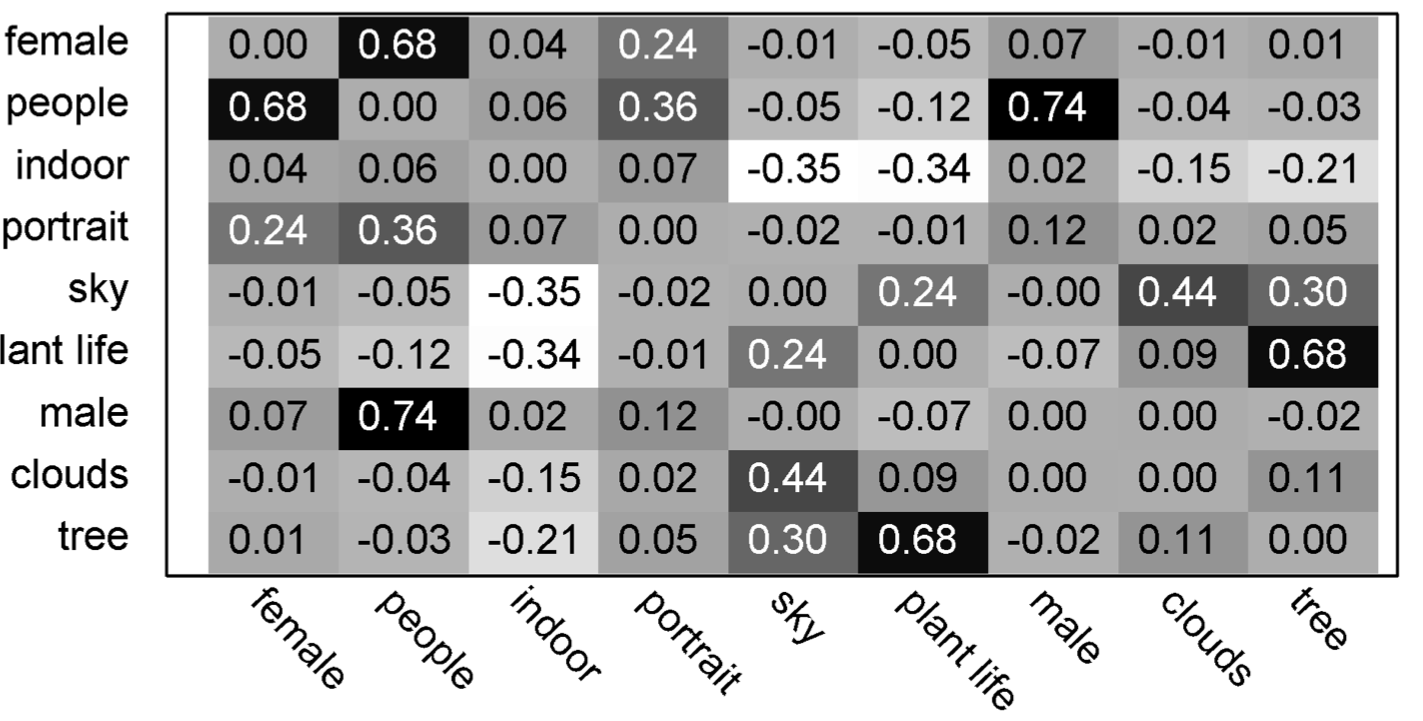
\includegraphics[scale=0.2]{img/flicker3}
	\end{center}
\end{frame}

\subsection*{Word Prediction}
\begin{frame}
	\begin{itemize}
		\item \textbf{Task}: Find five letters within distorted images, IYI = $26^5$
			\begin{center}
				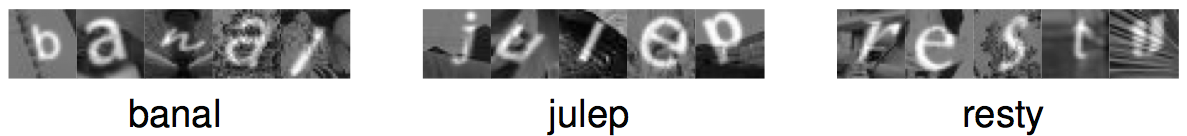
\includegraphics[scale=0.25]{img/words1}
			\end{center}
			
		\item \textbf{Graphical Model}:
			\begin{center}
				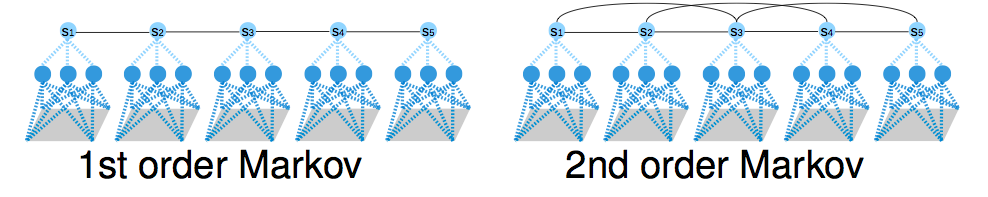
\includegraphics[scale=0.3]{img/words2}
			\end{center}
				
		\item \textbf{First order potential}: 
		\begin{enumerate}
			\item One Layer~: $f_i(x, y_i; U) = ReLu(U_1^T \cdot x)$
			\item Two Layers: $f_i(x, y_i; U) = ReLu(U_2^T \cdot ReLu(U_1^T \cdot x))$
		\end{enumerate}
		\item \textbf{Second order potential}: 
		\begin{enumerate}
			\item Linear: $f_{i, j}(x, y_i, y_j; W) = W_{y_iy_j}$
		\end{enumerate}
	\end{itemize}
\end{frame}

\begin{frame}
	\begin{center}		
		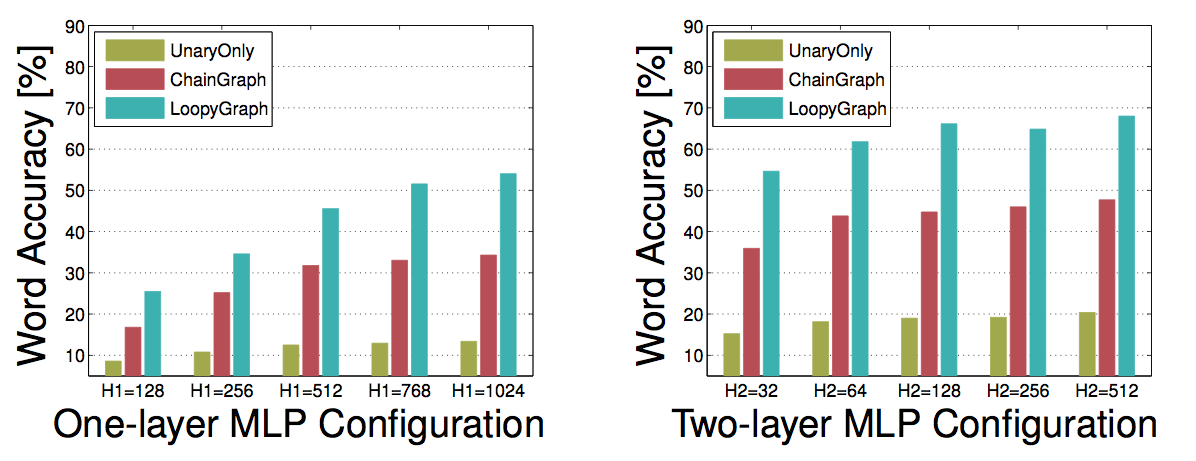
\includegraphics[scale=0.28]{img/words3}
	\end{center}		
\end{frame}

\subsection*{Semantic Segmentation [Raquel slides]}
	\begin{frame}
			\begin{itemize}
				\item \textbf{Task}: Image segmentation
				\item \textbf{Graphical Model}: Fully connected CRF with Gaussian potentials
				\item \textbf{NN}: PreTrain OxfordNet , predicts 40 $\times$ 40 + upsampling
				\item \textbf{Inference}: using (algo1), with mean-field as approx. inference
			\end{itemize}
			
			\begin{columns}[onlytextwidth]
				\begin{column}{0.5\textwidth}
					\begin{center}
						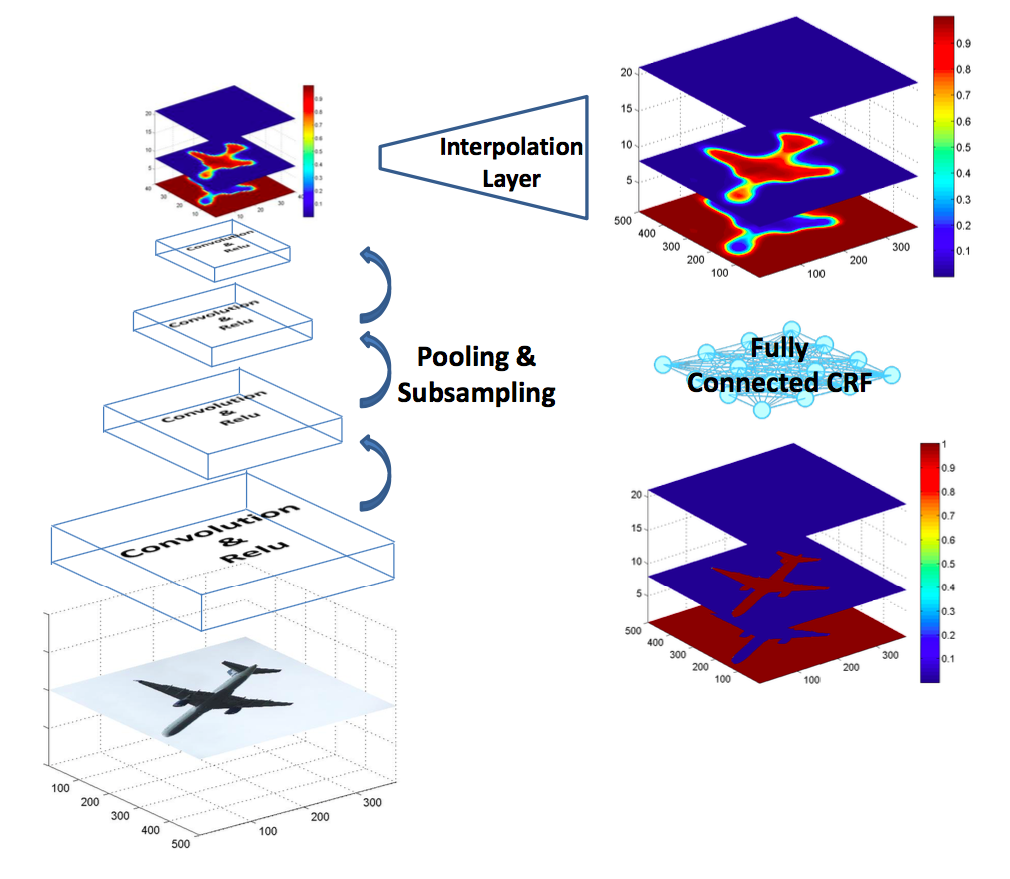
\includegraphics[scale=0.17]{img/ex3}
					\end{center}
				\end{column}
				\begin{column}{0.5\textwidth}
					\begin{center}
						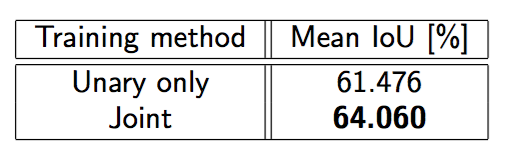
\includegraphics[scale=0.28]{img/ex3_1}
					\end{center}
				\end{column}
			\end{columns}
	\end{frame}

	\begin{frame}
		\centering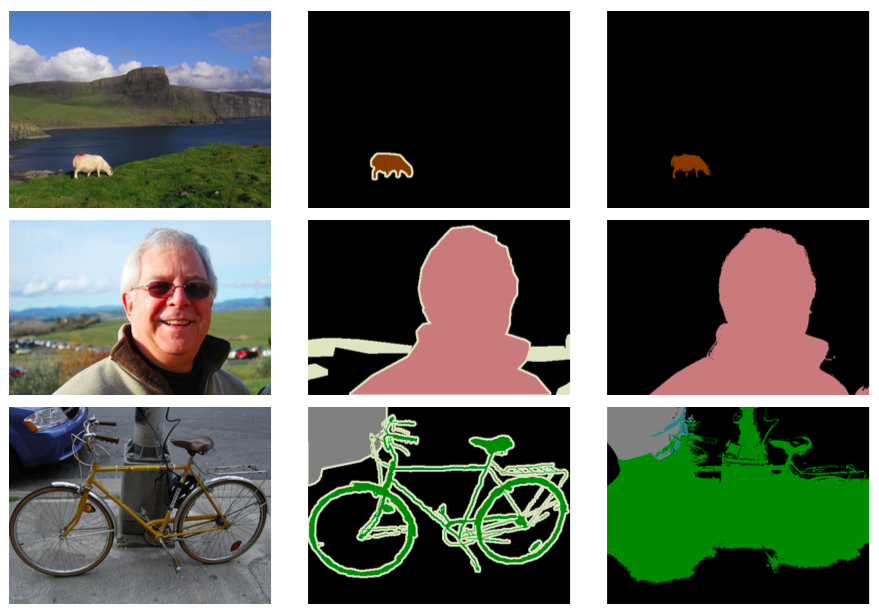
\includegraphics[scale=0.37]{img/ex3_2}
	\end{frame}
					
\subsection*{Summary}

\begin{frame}
		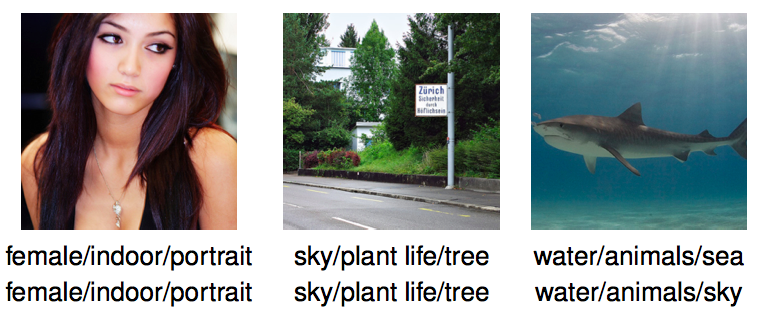
\includegraphics[scale=0.1]{img/flicker1}
		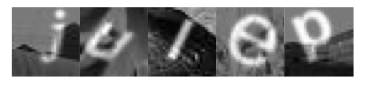
\includegraphics[scale=0.38]{img/words_11}
		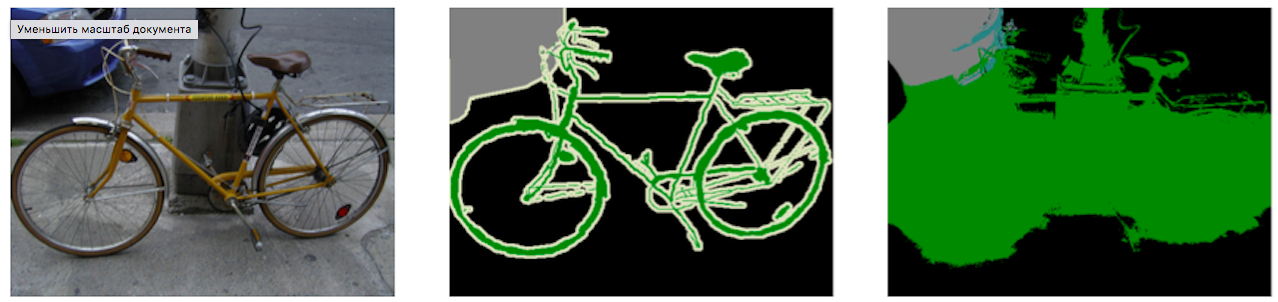
\includegraphics[scale=0.1]{img/ex3_4}
		\bigskip
		\begin{enumerate}
			\item Jointly learning helps
			\item Non-linear pairwise function improves over the linear one
			\item Deeper and more structured $\rightarrow$ better performance
			\item Wide range of applications: Word recognition, Tagging, Segmentation
		\end{enumerate}
\end{frame}

\section*{Bibliography}
\begin{frame}
	\begin{thebibliography}{10}
		\beamertemplatebookbibitems
		
		\bibitem{A} 
			\textcolor{black}{Chen, Schwing, Learning Deep Structured Models} \href{arxiv.org/pdf/1407.2538v1.pdf}{v1} \href{arxiv.org/pdf/1407.2538v2.pdf}{v2} \href{arxiv.org/pdf/1407.2538v3.pdf}{v3} \href{http://www.cs.toronto.edu/~urtasun/publications/chen_etal_icml15.pdf}{icml}
		
		\bibitem{C}
			\textcolor{black}{Hazan, Schwing, Blending Learning and Infer. in Struct. Pred.} \href{http://arxiv.org/pdf/1210.2346v2.pdf}{paper}
				
		\setbeamertemplate{bibliography item}[online]
		\bibitem{R} 	
			\textcolor{black}{Raquel Urtasun, CS Department, UofT, Learning Deep SM} \href{http://www.cs.toronto.edu/~urtasun/deep_structured_sports_small.pdf}{slides}
		
		\bibitem{D} 
			\textcolor{black}{Liang-Chieh Chen, CS Department, UofC, ICML} \href{http://videolectures.net/icml2015_chen_deep_structured_models}{video}  \href{http://videolectures.net/site/normal_dl/tag=1004999/icml2015_chen_deep_structured_models_01.pdf}{slides}
		
		\bibitem{D}
			\textcolor{black}{Alexandr Schwing, CS Department, UofT, Re.Work} \href{https://youtu.be/barVVAmXQPQ}{video}
	\end{thebibliography}
\end{frame}

\end{document}

